\section{State space transformation}

When transitioning from an analog system model to its discrete-time counterpart, we employ the following approach. 
\begin{figure}[H]
    \centering
    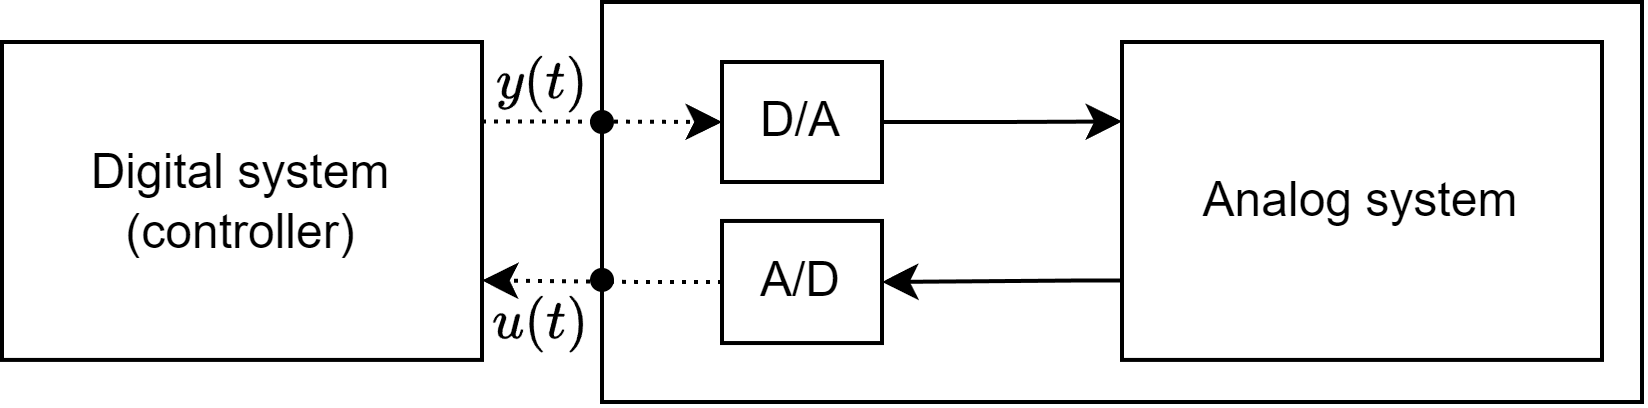
\includegraphics[width=0.5\linewidth]{images/sys.png}
    \caption{System}
\end{figure}
Beginning with a continuous model:
\[\mathcal{S}:\begin{cases} \dot{x}=Ax+Bu \\ y=Cx+Du \end{cases}\]
Assuming a sampling time of $\Delta T$: 
\[\mathcal{S}:\begin{cases} x(t+1)=Fx(t)+Gu(t) \\ y(t)=Hx(t)+Du(t) \end{cases}\]
The commonly used discretization method involves state space transformation:
\[F=e^{A\Delta T} \qquad G=\int_0^{\delta T}e^{A\delta}B \,d\delta\qquad H=C \qquad D=D\]

\paragraph*{Poles discretization}
The poles of the continuous-time system are discretized into discrete time using the sampling transformation rule $\mathcal{Z}=e^{\mathcal{S}\Delta T}$, and so we have: 
\[\lambda_F=e^{\lambda_A\Delta T}\]
Here, $\lambda_F$ represents the eigenvalues of matrix $F$, and $\lambda_A$ denotes the eigenvalues of matrix $A$.

\paragraph*{Zeros discretization}
Beginning with the transfer function in continuous time:
\[G(s)=\dfrac{\text{polynomial in }s\text{ with }h \text{ zeros}}{\text{polynomial in }s\text{ with }n \text{ poles}}\]
Where $h<n$. 
n discrete time, we have:
\[G(z)=\dfrac{\text{polynomial in }z\text{ with }n-1 \text{ zeros}}{\text{polynomial in }z\text{ with }n \text{ poles}}\]
During the transformation of zeros from continuous to discrete time, $n-h-1$ new zeros are generated, known as hidden zeros.
Unfortunately, these hidden zeros do not adhere to the sampling rule and are typically non-minimum phase.